\documentclass[11pt]{article}
\usepackage[a4paper,margin=0.88in]{geometry}
\usepackage{amsmath,amssymb,amsthm,mathtools}
\usepackage{graphicx}
\usepackage[hidelinks]{hyperref}
\usepackage{microtype}

\newtheorem{theorem}{Theorem}
\newtheorem{corollary}{Corollary}
\newcommand{\C}{\mathbb C}

\title{The smooth spherical-wavelet asymptotic,\\
and a phase counterexample to the literal formula}
\author{Candidate full-result packet for arXiv:2012.13460}
\date{17 August 2026}

\begin{document}
\maketitle

\begin{abstract}
Remark~7.4 of Dahlke--De Mari--De Vito--Hansen--Hasannasab--Quellmalz--
Steidl--Teschke conjectures an asymptotic for a zonal spherical-wavelet
coefficient and identifies the missing ingredient as an integrable bound after
the rescaling \(c=\ell a\).  We supply that bound for every axisymmetric
\(\eta\in C_c^\infty((0,\pi);\C)\) satisfying the paper's cancellation
condition.  The resulting formula has an absolute square on the right.  For
real-valued profiles this proves the displayed conjecture on a natural strong
regularity class.  For complex-valued profiles the ordinary square printed in
both the arXiv and published versions is false: multiplication by \(i\) leaves
the left side invariant and reverses the sign of the right side.
\end{abstract}

\paragraph{Status and scope.}
The positive theorem below assumes axisymmetry, smoothness, and compact support
away from the two poles.  It does not claim the weakest possible hypotheses.
The phase counterexample, however, is a complete disproof of the formula as
written on the paper's complex \(L_2\)-space, even under these very strong
regularity assumptions.  Equivalently, the displayed conjecture is correct in
this class for real profiles and becomes correct for complex profiles after
replacing the final square by an absolute square.

\section{Statement}

Use the notation of the source paper: \(D_a\) is its spherical dilation,
\(\eta_a=D_a\eta\), \(Y_\ell^0\) is the normalized zonal spherical harmonic,
and \(\kappa_0(\theta)=\tan(\theta/2)\).  For an axisymmetric profile, its
zonal average \(\widetilde\eta\) is simply \(\eta\).

\begin{theorem}[Smooth corrected form of Remark 7.4]\label{thm:limit}
Let \(\eta\in C_c^\infty((0,\pi);\C)\) be axisymmetric and satisfy
\begin{equation}\label{eq:cancel}
  \int_0^\pi \tan(\theta/2)\eta(\theta)\,d\theta=0.
\end{equation}
Then
\begin{align}\label{eq:limit}
 \lim_{\ell\to\infty}\frac1{2\ell+1}
 \int_0^\infty |\langle Y_\ell^0,\eta_a\rangle|^2\,\frac{da}{a^3}
 =4\pi\int_0^\infty\left|
 \int_0^\pi \tan(\theta/2)J_0\!\left(2c\tan(\theta/2)\right)
 \eta(\theta)\,d\theta\right|^2\frac{dc}{c}.
\end{align}
The integral on the right is finite.  It is strictly positive when
\(\eta\ne0\).
\end{theorem}

For real \(\eta\), the absolute square in \eqref{eq:limit} is the ordinary
square printed in Remark~7.4, so this is an affirmative result for that
conjecture under explicit stronger assumptions.

\section{Idea of the proof}

Put \(t=\tan(\theta/2)\), so the support of \(\eta\) becomes a compact interval
\([r,R]\Subset(0,\infty)\), and rescale \(a=c/\ell\).  The source already proves
pointwise convergence of the inner integral to a Hankel transform.  What is
needed is tightness in the logarithmic measure \(dc/c\).

There are four regimes.  Cancellation makes the inner integral \(O(c^2)\)
near \(c=0\).  Up to \(c=\delta\ell\), the uniform Hilb formula turns the
Legendre polynomial into an oscillatory Bessel function; integration by parts
gives arbitrary inverse powers of \(c\), apart from a harmless
\(O(\ell^{-3/2})\) remainder.  When \(c/\ell\) stays in a compact subinterval
of \((0,\infty)\), the phase is nonstationary at frequency \(\ell\).  Finally,
for \(c/\ell\) large, the elementary dilation amplitude is \(O((\ell/c)^2)\).
These estimates exactly close the gap stated by the authors.

\section{Proof of the asymptotic}

\begin{proof}[Proof of Theorem~\ref{thm:limit}]
Set
\[
 h(t)=\eta(2\arctan t),\qquad
 A(t,a)=\frac{2t}{(1+t^2)(1+a^2t^2)},\qquad
 z(t,a)=2\arctan(at).
\]
The calculation in Steps 1--2 of the source proof of Theorem~7.3, with
absolute values retained for complex functions, gives
\begin{align}
 \frac1{2\ell+1}\int_0^\infty
 |\langle Y_\ell^0,\eta_a\rangle|^2\frac{da}{a^3}
 &=4\pi\int_0^\infty |I_\ell(a)|^2\frac{da}{a},\label{eq:normal}\\
 I_\ell(a)&=\int_r^R A(t,a)P_\ell(\cos z(t,a))h(t)\,dt.\label{eq:I}
\end{align}
Here \(h\) is extended by zero, so it and all its derivatives vanish at the
chosen endpoints.  Condition \eqref{eq:cancel} becomes
\begin{equation}\label{eq:I0}
 I_\ell(0)=\int_r^R \frac{2t}{1+t^2}h(t)\,dt=0.
\end{equation}
After \(a=c/\ell\), define
\[
 F(c)=\int_r^R\frac{2t}{1+t^2}J_0(2ct)h(t)\,dt.
\]
The Mehler--Heine/Hilb limit used in the source yields
\begin{equation}\label{eq:pointwise}
 I_\ell(c/\ell)\longrightarrow F(c)
 \quad\text{for every fixed }c>0.
\end{equation}

We now prove the missing uniform tightness.  First, the standard bounds are
\[
 \|P_\ell\|_{L_\infty[-1,1]}\le1,\qquad
 \|P_\ell'\|_\infty\le\ell^2,
\]
the second being Markov's inequality.  Since
\[
 1-\cos z(t,a)=\frac{2a^2t^2}{1+a^2t^2},
 \qquad A(t,a)-A(t,0)=O(a^2)
\]
uniformly on \([r,R]\), equations \eqref{eq:I0}--\eqref{eq:I} imply
\begin{equation}\label{eq:small}
 |I_\ell(c/\ell)|\le Cc^2,\qquad 0<c\le1.
\end{equation}

Second, the uniform Hilb formula quoted in the source is
\begin{equation}\label{eq:hilb}
 P_\ell(\cos z)=\left(\frac z{\sin z}\right)^{1/2}
 J_0((\ell+\tfrac12)z)+O_\varepsilon(\ell^{-3/2}),
 \qquad 0\le z\le\pi-\varepsilon.
\end{equation}
For \(q\ge1\), write the standard Bessel expansion as
\[
 J_0(q)=e^{iq}b_+(q)+e^{-iq}b_-(q),\qquad
 |b_\pm^{(k)}(q)|\le C_kq^{-1/2-k}.
\]
Choose \(\delta>0\) with \(2\arctan(\delta R)<\pi/2\).  If
\(1\le c\le\delta\ell\), then the phase
\[
 \Phi_{\ell,c}(t)=(\ell+\tfrac12)z(t,c/\ell)
\]
satisfies \(\Phi'_{\ell,c}(t)\asymp c\), uniformly on \([r,R]\); all normalized
phase and amplitude derivatives are uniform as well.  Repeated integration by
parts in the two exponentials, followed by \eqref{eq:hilb}, gives, for every
\(N\),
\begin{equation}\label{eq:lowtail}
 |I_\ell(c/\ell)|\le C_Nc^{-N}+C\ell^{-3/2},\qquad
 1\le c\le\delta\ell.
\end{equation}

Fix \(A>\delta\).  When \(\delta\ell\le c\le A\ell\), the parameter
\(a=c/\ell\) lies in \([\delta,A]\).  Hence \(z(t,a)\) stays in a compact
subinterval of \((0,\pi)\), and
\[
 \partial_t z(t,a)=\frac{2a}{1+a^2t^2}
\]
is uniformly separated from zero.  One integration by parts in the Bessel
waves in \eqref{eq:hilb}, including their \(q^{-1/2}\) amplitude, gives
\begin{equation}\label{eq:middle}
 |I_\ell(c/\ell)|\le C_A\ell^{-3/2},\qquad
 \delta\ell\le c\le A\ell.
\end{equation}
For the remaining range, \(a=c/\ell\ge A\), the support condition \(t\ge r\),
\(|P_\ell|\le1\), and \eqref{eq:I} give the elementary bound
\begin{equation}\label{eq:far}
 |I_\ell(c/\ell)|\le Ca^{-2}=C(\ell/c)^2,\qquad c\ge A\ell.
\end{equation}

The limiting transform has the analogous endpoint bounds
\begin{equation}\label{eq:Fbounds}
 |F(c)|\le Cc^2\quad(0<c\le1),\qquad
 |F(c)|\le C_Nc^{-N}\quad(c\ge1).
\end{equation}
The first follows from cancellation and \(J_0(2ct)-1=O(c^2t^2)\); the second
follows from the same Bessel-wave integration by parts, since \(h\) is smooth
and compactly supported away from zero.  Thus \(|F(c)|^2/c\) is integrable.

For completeness, the estimates assemble as follows.  For \(M>1\),
\begin{align*}
 \limsup_{\ell\to\infty}\int_M^{\delta\ell}
 |I_\ell(c/\ell)|^2\frac{dc}{c}&\le C_NM^{-2N},\\
 \int_{\delta\ell}^{A\ell}|I_\ell(c/\ell)|^2\frac{dc}{c}
 &\le C_A\ell^{-3}\log(A/\delta)\longrightarrow0,\\
 \int_{A\ell}^{\infty}|I_\ell(c/\ell)|^2\frac{dc}{c}&\le CA^{-4}.
\end{align*}
On \((0,M]\), equations \eqref{eq:pointwise} and \eqref{eq:small} give
dominated convergence (split once at \(c=1\)).  Let first \(\ell\to\infty\),
then \(M\to\infty\), and finally \(A\to\infty\).  We obtain
\[
 \int_0^\infty|I_\ell(c/\ell)|^2\frac{dc}{c}
 \longrightarrow \int_0^\infty|F(c)|^2\frac{dc}{c}.
\]
Together with \eqref{eq:normal}, this proves \eqref{eq:limit}.

Finally, put \(g(t)=2h(t)/(1+t^2)\).  Then
\(F(c)=\int_0^\infty tg(t)J_0(2ct)\,dt\).  Injectivity (or Parseval's theorem)
for the order-zero Hankel transform shows that \(F\not\equiv0\) whenever
\(\eta\not\equiv0\).  Continuity of \(F\) then makes the right side of
\eqref{eq:limit} strictly positive.
\end{proof}

\section{A full counterexample to the printed complex formula}

\begin{corollary}\label{cor:phase}
There is a nonzero axisymmetric
\(\eta\in C_c^\infty((0,\pi);\C)\) satisfying every explicit assumption of
the source theorem and its cancellation condition, for which the equality
printed in Remark~7.4 is false.
\end{corollary}

\begin{proof}
Choose nonzero nonnegative \(u,v\in C_c^\infty((0,\pi);\mathbb R)\) with
disjoint supports, and set
\[
 m_u=\int_0^\pi\tan(\theta/2)u(\theta)\,d\theta,
 \quad m_v=\int_0^\pi\tan(\theta/2)v(\theta)\,d\theta,
 \quad \eta_0=u-\frac{m_u}{m_v}v.
\]
Then \(m_u,m_v>0\), \(\eta_0\ne0\), and \eqref{eq:cancel} holds.  By
Theorem~\ref{thm:limit}, its absolute-square Hankel energy is a finite number
\(R>0\).

Take \(\eta=i\eta_0\).  Every term on the left of the printed conjecture is
unchanged, since
\[
 |\langle Y_\ell^0,i(\eta_0)_a\rangle|^2
 =|\langle Y_\ell^0,(\eta_0)_a\rangle|^2.
\]
Its limit is therefore \(R\).  But the ordinary-square right side printed in
the paper is
\[
 4\pi\int_0^\infty(iF_0(c))^2\frac{dc}{c}=-R<0.
\]
Thus the two sides cannot agree.  The obstruction is removed either by
assuming \(\eta\) real-valued or by printing an absolute square.
\end{proof}

\section{Source evidence}

The published-author PDF states the missing domination issue and displays the
ordinary square in Remark~7.4 (PDF page 23):
\begin{center}
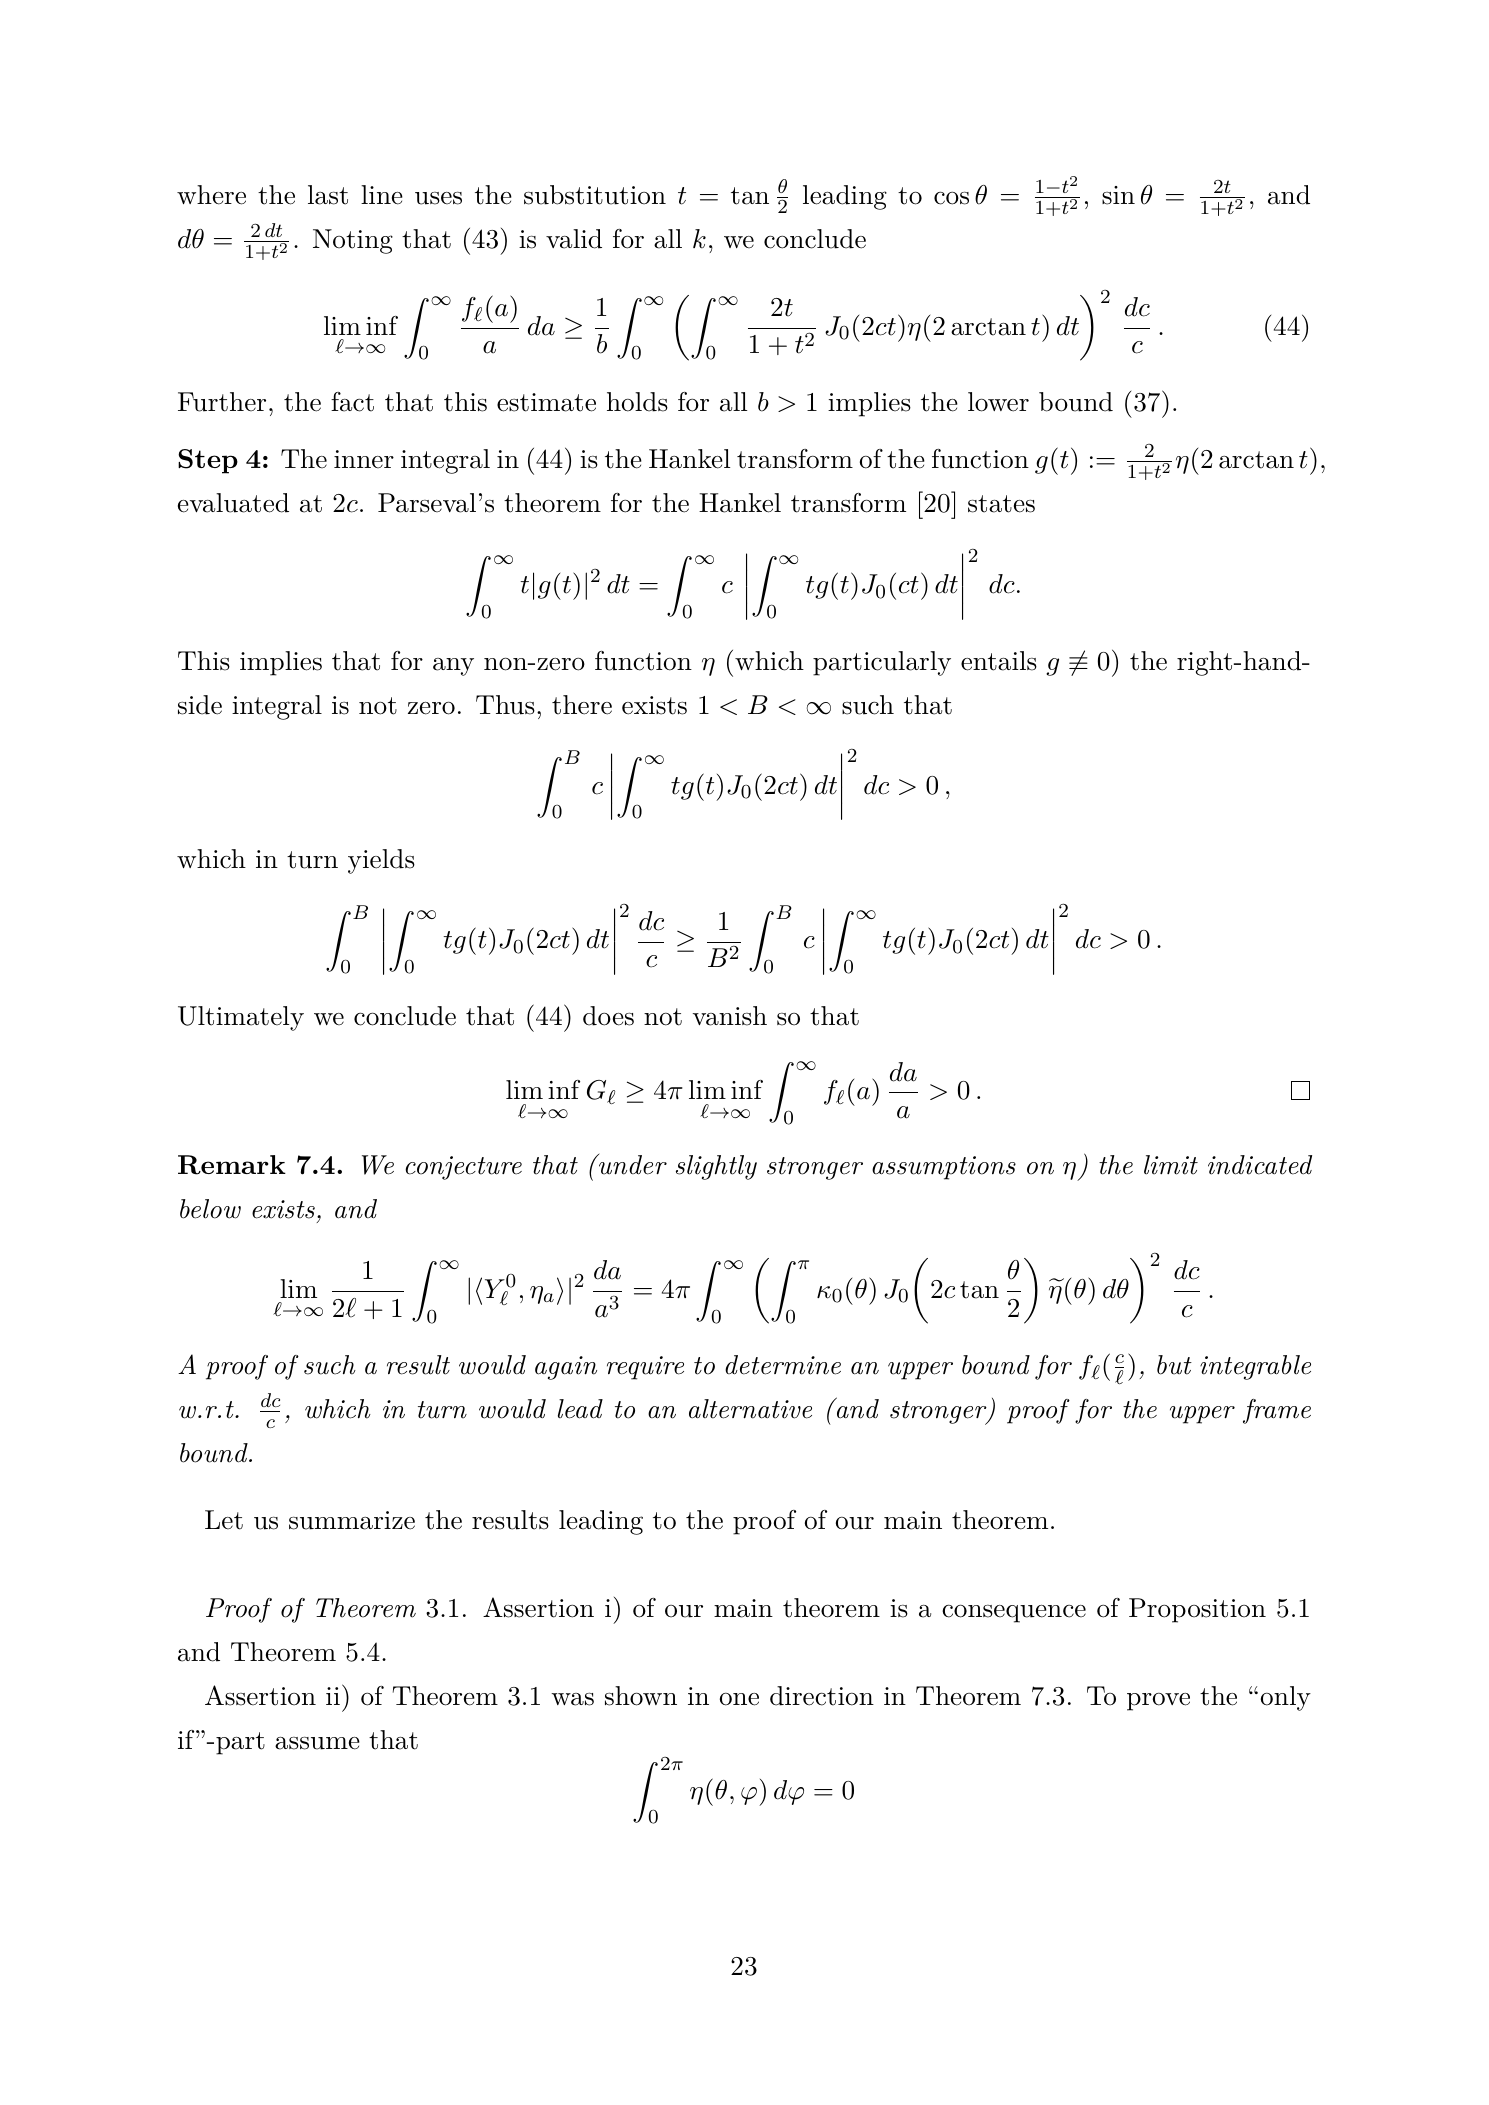
\includegraphics[width=0.96\linewidth,trim=45bp 245bp 45bp 315bp,clip]
 {figures/source_page_23.png}
\end{center}

\begin{thebibliography}{9}
\bibitem{source}
S.~Dahlke, F.~De Mari, E.~De Vito, M.~Hansen, M.~Hasannasab,
M.~Quellmalz, G.~Steidl, and G.~Teschke,
\emph{Continuous Wavelet Frames on the Sphere: The Group-Theoretic Approach
Revisited}, Appl. Comput. Harmon. Anal. \textbf{56} (2022), 123--149;
arXiv:2012.13460.  See Theorem~7.3 and Remark~7.4.

\bibitem{szego}
G.~Szeg\H{o}, \emph{Orthogonal Polynomials}, 4th ed., American Mathematical
Society, 1975, Theorem~8.21.6 (the uniform Hilb formula used by the source).

\bibitem{macaulay}
P.~MacAulay-Owen, \emph{Parseval's theorem for Hankel transforms},
Proc. London Math. Soc. \textbf{45} (1939), 458--474.
\end{thebibliography}

\end{document}
